%Chapter 10
\chapter{Listas}

Este capítulo presenta uno de los tipos integrados más útiles de Python: las listas. También aprenderás más sobre objetos y lo que puede suceder cuando tienes más de un nombre para el mismo objeto.

\section{Una lista es una secuencia}

Al igual que una cadena, una lista es una secuencia de valores. En una cadena, los valores son caracteres; en una lista, pueden ser de cualquier tipo. Los valores en una lista se llaman \textbf{elementos} o, a veces, \textbf{ítems}.

Hay varias formas de crear una nueva lista; la más simple es encerrar los elementos entre corchetes ([ y ]):

\begin{lstlisting}[language=Python]
[10, 20, 30, 40]  
['crunchy frog', 'ram bladder', 'lark vomit']  
\end{lstlisting}

El primer ejemplo es una lista de cuatro enteros. El segundo es una lista de tres cadenas. Los elementos de una lista no tienen que ser del mismo tipo. La siguiente lista contiene una cadena, un flotante, un entero y (¡oh!) otra lista:

\begin{lstlisting}[language=Python]
['spam', 2.0, 5, [10, 20]]
\end{lstlisting}

Una lista dentro de otra lista se llama \textbf{lista anidada}.

Una lista que no contiene elementos se llama \textbf{lista vacía}; puedes crear una con corchetes vacíos, [].

Como era de esperar, puedes asignar valores de lista a variables:

\begin{lstlisting}[language=Python]
>>> cheeses = ['Cheddar', 'Edam', 'Gouda']  
>>> numbers = [42, 123]  
>>> empty = []  

>>> print(cheeses, numbers, empty)  
['Cheddar', 'Edam', 'Gouda'] [42, 123]
\end{lstlisting}
\begin{figure}[h]
        \centering
        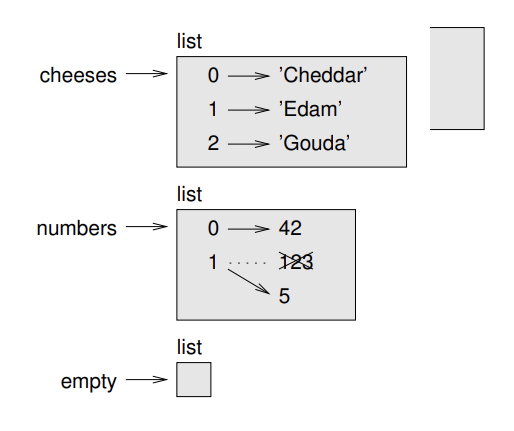
\includegraphics[width=0.5\textwidth]{./images/chapter_10_1.png}
        \caption{Diagrama de estados.}
        \label{fig:10_1}
        \end{figure}
\section{Las listas son mutables}

La sintaxis para acceder a los elementos de una lista es la misma que para acceder a los caracteres de una cadena: el operador de corchetes. La expresión dentro de los corchetes especifica el índice. Recuerda que los índices comienzan en 0:

\begin{lstlisting}[language=Python]
>>> cheeses[0] 
'Cheddar'
\end{lstlisting}

A diferencia de las cadenas, las listas son mutables. Cuando el operador de corchetes aparece en el lado izquierdo de una asignación, identifica el elemento de la lista que será asignado.

\begin{lstlisting}[language=Python]
>>> numbers = [42, 123] 
>>> numbers[1] = 5 
>>> numbers 
[42, 5]
\end{lstlisting}

El elemento en la posición 1 de \texttt{numbers}, que solía ser 123, ahora es 5.

Los índices de lista funcionan de la misma manera que los índices de cadena:

\begin{itemize}
    \item Cualquier expresión entera puede usarse como índice.
    \item Si intentas leer o escribir un elemento que no existe, obtienes un \texttt{IndexError}.
    \item Si un índice tiene un valor negativo, cuenta hacia atrás desde el final de la lista.
\end{itemize}

El operador \texttt{in} también funciona con listas.

\begin{lstlisting}[language=Python]
>>> cheeses = ['Cheddar', 'Edam', 'Gouda'] 
>>> 'Edam' in cheeses 
True 
>>> 'Brie' in cheeses 
False
\end{lstlisting}

\section{Recorriendo una lista}

La forma más común de recorrer los elementos de una lista es con un bucle \texttt{for}. La sintaxis es la misma que para cadenas:

\begin{lstlisting}[language=Python]
for cheese in cheeses:
    print(cheese)
\end{lstlisting}

Esto funciona bien si solo necesitas leer los elementos de la lista. Pero si quieres escribir o actualizar los elementos, necesitas los índices. Una forma común de hacerlo es combinar las funciones integradas \texttt{range} y \texttt{len}:

\begin{lstlisting}[language=Python]
for i in range(len(numbers)):
    numbers[i] = numbers[i] * 2
\end{lstlisting}

Este bucle recorre la lista y actualiza cada elemento. \texttt{len} devuelve el número de elementos en la lista. \texttt{range} devuelve una lista de índices desde 0 hasta \(n-1\), donde \(n\) es la longitud de la lista. Cada vez que se ejecuta el bucle, \texttt{i} obtiene el índice del siguiente elemento. La declaración de asignación en el cuerpo usa \texttt{i} para leer el valor antiguo del elemento y asignar el nuevo valor.

Un bucle \texttt{for} sobre una lista vacía nunca ejecuta el cuerpo:

\begin{lstlisting}[language=Python]
for x in []:
    print('This never happens.')
\end{lstlisting}

Aunque una lista puede contener otra lista, la lista anidada todavía cuenta como un solo elemento. La longitud de esta lista es cuatro:

\begin{lstlisting}[language=Python]
['spam', 1, ['Brie', 'Roquefort', 'Pol le Veq'], [1, 2, 3]]
\end{lstlisting}

\section{Operaciones con listas}

El operador \texttt{+} concatena listas:

\begin{lstlisting}[language=Python]
>>> a = [1, 2, 3] 
>>> b = [4, 5, 6] 
>>> c = a + b 
>>> c 
[1, 2, 3, 4, 5, 6]
\end{lstlisting}

El operador \texttt{*} repite una lista un número determinado de veces:

\begin{lstlisting}[language=Python]
>>> [0] * 4 
[0, 0, 0, 0] 
>>> [1, 2, 3] * 3 
[1, 2, 3, 1, 2, 3, 1, 2, 3]
\end{lstlisting}

El primer ejemplo repite \texttt{[0]} cuatro veces. El segundo ejemplo repite la lista \texttt{[1, 2, 3]} tres veces.

\section{Segmentos de lista}

El operador de segmento también funciona con listas:

\begin{lstlisting}[language=Python]
>>> t = ['a', 'b', 'c', 'd', 'e', 'f'] 
>>> t[1:3] 
['b', 'c'] 
>>> t[:4] 
['a', 'b', 'c', 'd'] 
>>> t[3:] 
['d', 'e', 'f']
\end{lstlisting}

Si omites el primer índice, el segmento comienza al principio. Si omites el segundo, el segmento va hasta el final. Si omites ambos, el segmento es una copia de toda la lista.

\begin{lstlisting}[language=Python]
>>> t[:] 
['a', 'b', 'c', 'd', 'e', 'f']
\end{lstlisting}

Dado que las listas son mutables, a menudo es útil hacer una copia antes de realizar operaciones que modifiquen listas.

Un operador de segmento en el lado izquierdo de una asignación puede actualizar múltiples elementos:

\begin{lstlisting}[language=Python]
>>> t = ['a', 'b', 'c', 'd', 'e', 'f'] 
>>> t[1:3] = ['x', 'y'] 
>>> t 
['a', 'x', 'y', 'd', 'e', 'f']
\end{lstlisting}

\section{Métodos de lista}

Python proporciona métodos que operan en listas. Por ejemplo, \texttt{append} agrega un nuevo elemento al final de una lista:

\begin{lstlisting}[language=Python]
>>> t = ['a', 'b', 'c'] 
>>> t.append('d') 
>>> t 
['a', 'b', 'c', 'd']
\end{lstlisting}

\texttt{extend} toma una lista como argumento y agrega todos sus elementos:

\begin{lstlisting}[language=Python]
>>> t1 = ['a', 'b', 'c'] 
>>> t2 = ['d', 'e'] 
>>> t1.extend(t2) 
>>> t1 
['a', 'b', 'c', 'd', 'e']
\end{lstlisting}

Este ejemplo deja \texttt{t2} sin modificar.

\texttt{sort} ordena los elementos de la lista de menor a mayor:

\begin{lstlisting}[language=Python]
>>> t = ['d', 'c', 'e', 'b', 'a'] 
>>> t.sort() 
>>> t 
['a', 'b', 'c', 'd', 'e']
\end{lstlisting}

La mayoría de los métodos de lista son nulos; modifican la lista y devuelven \texttt{None}. Si accidentalmente escribes \texttt{t = t.sort()}, te decepcionará el resultado.

\section{Map, filter y reduce}

Para sumar todos los números en una lista, puedes usar un bucle como este:

\begin{lstlisting}[language=Python]
def add_all(t):
    total = 0
    for x in t:
        total += x
    return total
\end{lstlisting}

\texttt{total} se inicializa en 0. Cada vez que se ejecuta el bucle, \texttt{x} obtiene un elemento de la lista. El operador \texttt{+=} proporciona una forma abreviada de actualizar una variable. Esta declaración de asignación aumentada,

\begin{lstlisting}[language=Python]
total += x
\end{lstlisting}

es equivalente a

\begin{lstlisting}[language=Python]
total = total + x
\end{lstlisting}

A medida que se ejecuta el bucle, \texttt{total} acumula la suma de los elementos; una variable usada de esta manera a veces se llama \textbf{acumulador}.

Sumar los elementos de una lista es una operación tan común que Python la proporciona como una función integrada, \texttt{sum}:

\begin{lstlisting}[language=Python]
>>> t = [1, 2, 3] 
>>> sum(t) 
6
\end{lstlisting}

Una operación como esta que combina una secuencia de elementos en un solo valor a veces se llama \textbf{reduce}.

A veces quieres recorrer una lista mientras construyes otra. Por ejemplo, la siguiente función toma una lista de cadenas y devuelve una nueva lista que contiene las cadenas en mayúsculas:

\begin{lstlisting}[language=Python]
def capitalize_all(t):
    res = []
    for s in t:
        res.append(s.capitalize())
    return res
\end{lstlisting}

\texttt{res} se inicializa con una lista vacía; cada vez que se ejecuta el bucle, agregamos el siguiente elemento. Así que \texttt{res} es otro tipo de acumulador.

Una operación como \texttt{capitalize\_all} a veces se llama \textbf{map} porque "mapea" una función (en este caso, el método \texttt{capitalize}) sobre cada uno de los elementos en una secuencia.

Otra operación común es seleccionar algunos elementos de una lista y devolver una sublista. Por ejemplo, la siguiente función toma una lista de cadenas y devuelve una lista que contiene solo las cadenas en mayúsculas:

\begin{lstlisting}[language=Python]
def only_upper(t):
    res = []
    for s in t:
        if s.isupper():
            res.append(s)
    return res
\end{lstlisting}

\texttt{isupper} es un método de cadena que devuelve \texttt{True} si la cadena contiene solo letras mayúsculas. Una operación como \texttt{only\_upper} se llama \textbf{filter} porque selecciona algunos de los elementos y filtra los demás. La mayoría de las operaciones comunes de listas se pueden expresar como una combinación de \texttt{map}, \texttt{filter} y \texttt{reduce}.

\section{Eliminando elementos}

Hay varias formas de eliminar elementos de una lista. Si conoces el índice del elemento que deseas eliminar, puedes usar \texttt{pop}:

\begin{lstlisting}[language=Python]
>>> t = ['a', 'b', 'c'] 
>>> x = t.pop(1) 
>>> t 
['a', 'c'] 
>>> x 
'b'
\end{lstlisting}

\texttt{pop} modifica la lista y devuelve el elemento que fue eliminado. Si no proporcionas un índice, elimina y devuelve el último elemento.

Si no necesitas el valor eliminado, puedes usar el operador \texttt{del}:

\begin{lstlisting}[language=Python]
>>> t = ['a', 'b', 'c'] 
>>> del t[1] 
>>> t 
['a', 'c']
\end{lstlisting}

Si conoces el elemento que deseas eliminar (pero no el índice), puedes usar \texttt{remove}:

\begin{lstlisting}[language=Python]
>>> t = ['a', 'b', 'c'] 
>>> t.remove('b') 
>>> t 
['a', 'c']
\end{lstlisting}

El valor de retorno de \texttt{remove} es \texttt{None}.

Para eliminar más de un elemento, puedes usar \texttt{del} con un índice de segmento:

\begin{lstlisting}[language=Python]
>>> t = ['a', 'b', 'c', 'd', 'e', 'f'] 
>>> del t[1:5] 
>>> t 
['a', 'f']
\end{lstlisting}

Como es habitual, el segmento selecciona todos los elementos hasta, pero sin incluir, el segundo índice.

\section{Listas y cadenas}

Una cadena es una secuencia de caracteres y una lista es una secuencia de valores, pero una lista de caracteres no es lo mismo que una cadena. Para convertir una cadena en una lista de caracteres, puedes usar \texttt{list}:

\begin{lstlisting}[language=Python]
>>> s = 'spam' 
>>> t = list(s) 
>>> t 
['s', 'p', 'a', 'm']
\end{lstlisting}

\begin{figure}[h]
        \centering
        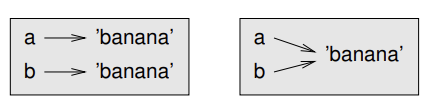
\includegraphics[width=0.5\textwidth]{./images/chapter_10_2.png}
        \caption{Diagrama de estados.}
        \label{fig:10_2}
        \end{figure}


Dado que \texttt{list} es el nombre de una función integrada, debes evitar usarlo como nombre de variable. También evito \texttt{l} porque se parece demasiado a \texttt{1}. Por eso uso \texttt{t}.

La función \texttt{list} divide una cadena en letras individuales. Si deseas dividir una cadena en palabras, puedes usar el método \texttt{split}:

\begin{lstlisting}[language=Python]
>>> s = 'pining for the fjords' 
>>> t = s.split() 
>>> t 
['pining', 'for', 'the', 'fjords']
\end{lstlisting}

Un argumento opcional llamado \textbf{delimitador} especifica qué caracteres usar como límites de palabras. El siguiente ejemplo usa un guión como delimitador:

\begin{lstlisting}[language=Python]
>>> s = 'spam-spam-spam' 
>>> delimiter = '-' 
>>> t = s.split(delimiter) 
>>> t 
['spam', 'spam', 'spam']
\end{lstlisting}

\texttt{join} es el inverso de \texttt{split}. Toma una lista de cadenas y concatena los elementos. \texttt{join} es un método de cadena, por lo que debes invocarlo en el delimitador y pasar la lista como parámetro:

\begin{lstlisting}[language=Python]
>>> t = ['pining', 'for', 'the', 'fjords'] 
>>> delimiter = ' ' 
>>> s = delimiter.join(t) 
>>> s 
'pining for the fjords'
\end{lstlisting}

En este caso, el delimitador es un espacio, por lo que \texttt{join} coloca un espacio entre las palabras. Para concatenar cadenas sin espacios, puedes usar la cadena vacía, \texttt{''}, como delimitador.

\section{Objetos y valores}

Si ejecutamos estas declaraciones de asignación:

\begin{lstlisting}[language=Python]
a = 'banana'
b = 'banana'
\end{lstlisting}

Sabemos que \texttt{a} y \texttt{b} se refieren a una cadena, pero no sabemos si se refieren a la misma cadena. Hay dos estados posibles:

En un caso, \texttt{a} y \texttt{b} se refieren a dos objetos diferentes que tienen el mismo valor. En el segundo caso, se refieren al mismo objeto.

Para verificar si dos variables se refieren al mismo objeto, puedes usar el operador \texttt{is}:
\begin{figure}[h]
        \centering
        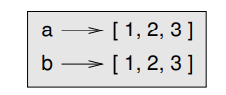
\includegraphics[width=0.5\textwidth]{./images/chapter_10_3.png}
        \caption{Diagrama de estados.}
        \label{fig:10_3}
        \end{figure}

\begin{figure}[h]
        \centering
        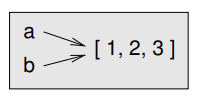
\includegraphics[width=0.5\textwidth]{./images/chapter_10_4.png}
        \caption{Diagrama de estados.}
        \label{fig:10_4}
        \end{figure}

\begin{lstlisting}[language=Python]
>>> a = 'banana' 
>>> b = 'banana' 
>>> a is b 
True
\end{lstlisting}

En este ejemplo, Python solo creó un objeto de cadena, y tanto \texttt{a} como \texttt{b} se refieren a él. Pero cuando creas dos listas, obtienes dos objetos:

\begin{lstlisting}[language=Python]
>>> a = [1, 2, 3] 
>>> b = [1, 2, 3] 
>>> a is b 
False
\end{lstlisting}

En este caso, diríamos que las dos listas son \textbf{equivalentes}, porque tienen los mismos elementos, pero no \textbf{idénticas}, porque no son el mismo objeto. Si dos objetos son idénticos, también son equivalentes, pero si son equivalentes, no son necesariamente idénticos.

Hasta ahora, hemos estado usando "objeto" y "valor" indistintamente, pero es más preciso decir que un objeto tiene un valor. Si evalúas \texttt{[1, 2, 3]}, obtienes un objeto de lista cuyo valor es una secuencia de enteros. Si otra lista tiene los mismos elementos, decimos que tiene el mismo valor, pero no es el mismo objeto.

\section{Alias}

Si \texttt{a} se refiere a un objeto y asignas \texttt{b = a}, entonces ambas variables se refieren al mismo objeto:

\begin{lstlisting}[language=Python]
>>> a = [1, 2, 3] 
>>> b = a 
>>> b is a 
True
\end{lstlisting}

La asociación de una variable con un objeto se llama \textbf{referencia}. En este ejemplo, hay dos referencias al mismo objeto.

Un objeto con más de una referencia tiene más de un nombre, por lo que decimos que el objeto tiene un \textbf{alias}.

Si el objeto con alias es mutable, los cambios realizados con un alias afectan al otro:

\begin{figure}[h]
        \centering
        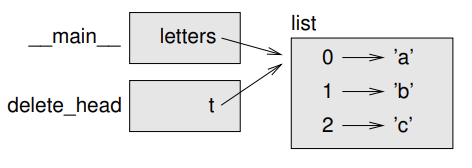
\includegraphics[width=0.5\textwidth]{./images/chapter_10_5.png}
        \caption{Diagrama de pila.}
        \label{fig:10_5}
        \end{figure}


\begin{lstlisting}[language=Python]
>>> b[0] = 42 
>>> a 
[42, 2, 3]
\end{lstlisting}

Aunque este comportamiento puede ser útil, es propenso a errores. En general, es más seguro evitar los alias cuando trabajas con objetos mutables.

Para objetos inmutables como cadenas, los alias no son un problema tan grande. En este ejemplo:

\begin{lstlisting}[language=Python]
a = 'banana'
b = 'banana'
\end{lstlisting}

Casi nunca importa si \texttt{a} y \texttt{b} se refieren a la misma cadena o no.

\section{Argumentos de lista}

Cuando pasas una lista a una función, la función obtiene una referencia a la lista. Si la función modifica la lista, el llamador ve el cambio. Por ejemplo, \texttt{delete\_head} elimina el primer elemento de una lista:

\begin{lstlisting}[language=Python]
def delete_head(t):
    del t[0]
\end{lstlisting}

Así es como se usa:

\begin{lstlisting}[language=Python]
>>> letters = ['a', 'b', 'c'] 
>>> delete_head(letters) 
>>> letters 
['b', 'c']
\end{lstlisting}

El parámetro \texttt{t} y la variable \texttt{letters} son alias para el mismo objeto.

Es importante distinguir entre operaciones que modifican listas y operaciones que crean nuevas listas. Por ejemplo, el método \texttt{append} modifica una lista, pero el operador \texttt{+} crea una nueva lista.

Aquí un ejemplo usando \texttt{append}:

\begin{lstlisting}[language=Python]
>>> t1 = [1, 2] 
>>> t2 = t1.append(3) 
>>> t1 
[1, 2, 3] 
>>> t2 
None
\end{lstlisting}

El valor de retorno de \texttt{append} es \texttt{None}.

Aquí un ejemplo usando el operador \texttt{+}:

\begin{lstlisting}[language=Python]
>>> t3 = t1 + [4] 
>>> t1 
[1, 2, 3] 
>>> t3 
[1, 2, 3, 4]
\end{lstlisting}

El resultado del operador es una nueva lista, y la lista original no cambia.

Esta diferencia es importante cuando escribes funciones que deben modificar listas. Por ejemplo, esta función \textbf{no} elimina la cabeza de una lista:

\begin{lstlisting}[language=Python]
def bad_delete_head(t):
    t = t[1:]  # !INCORRECTO
\end{lstlisting}


El operador de segmento crea una nueva lista y la asignación hace que \texttt{t} se refiera a ella, pero eso no afecta al llamador.

\begin{lstlisting}[language=Python]
>>> t4 = [1, 2, 3] 
>>> bad_delete_head(t4) 
>>> t4 
[1, 2, 3]
\end{lstlisting}

Al principio de \texttt{bad\_delete\_head}, \texttt{t} y \texttt{t4} se refieren a la misma lista. Al final, \texttt{t} se refiere a una nueva lista, pero \texttt{t4} todavía se refiere a la lista original sin modificar.

Una alternativa es escribir una función que cree y devuelva una nueva lista. Por ejemplo, \texttt{tail} devuelve todos los elementos excepto el primero de una lista:

\begin{lstlisting}[language=Python]
def tail(t):
    return t[1:]
\end{lstlisting}

Esta función deja la lista original sin modificar. Así es como se usa:

\begin{lstlisting}[language=Python]
>>> letters = ['a', 'b', 'c'] 
>>> rest = tail(letters) 
>>> rest 
['b', 'c']
\end{lstlisting}

\section{Depuración}

El uso descuidado de listas (y otros objetos mutables) puede llevar a largas horas de depuración. Aquí hay algunos errores comunes y formas de evitarlos:

\begin{enumerate}
    \item La mayoría de los métodos de lista modifican el argumento y devuelven \texttt{None}. Esto es lo opuesto a los métodos de cadena, que devuelven una nueva cadena y dejan el original intacto. Si estás acostumbrado a escribir código de cadena como este:
    
    \begin{lstlisting}[language=Python]
    word = word.strip()
    \end{lstlisting}
    
    Es tentador escribir código de lista como este:
    
    \begin{lstlisting}[language=Python]
    t = t.sort()  # !INCORRECTO
    \end{lstlisting}

    
    Debido a que \texttt{sort} devuelve \texttt{None}, la siguiente operación que realices con \texttt{t} probablemente fallará.
    
    Antes de usar métodos y operadores de lista, debes leer la documentación cuidadosamente y luego probarlos en modo interactivo.
    
    \item Elige un estilo y apégate a él.
    
    Parte del problema con las listas es que hay demasiadas formas de hacer las cosas. Por ejemplo, para eliminar un elemento de una lista, puedes usar \texttt{pop}, \texttt{remove}, \texttt{del} o incluso una asignación de segmento.
    
    Para agregar un elemento, puedes usar el método \texttt{append} o el operador \texttt{+}. Asumiendo que \texttt{t} es una lista y \texttt{x} es un elemento de lista, estos son correctos:
    
    \begin{lstlisting}[language=Python]
    t.append(x)
    t = t + [x]
    t += [x]
    \end{lstlisting}
    
    Y estos son incorrectos:
    
    \begin{lstlisting}[language=Python]
    t.append([x])     # ! INCORRECTO
    t = t.append(x)   # ! INCORRECTO
    t + [x]           # ! INCORRECTO
    t = t + x         # ! INCORRECTO
    \end{lstlisting}


    
    Prueba cada uno de estos ejemplos en modo interactivo para asegurarte de entender lo que hacen. Observa que solo el último causa un error en tiempo de ejecución; los otros tres son legales, pero hacen lo incorrecto.
    
    \item Haz copias para evitar alias.
    
    Si quieres usar un método como \texttt{sort} que modifica el argumento, pero necesitas mantener la lista original también, puedes hacer una copia.
    
    \begin{lstlisting}[language=Python]
    >>> t = [3, 1, 2] 
    >>> t2 = t[:] 
    >>> t2.sort() 
    >>> t 
    [3, 1, 2] 
    >>> t2 
    [1, 2, 3]
    \end{lstlisting}
    
    En este ejemplo, también podrías usar la función integrada \texttt{sorted}, que devuelve una nueva lista ordenada y deja la original intacta.
    
    \begin{lstlisting}[language=Python]
    >>> t2 = sorted(t) 
    >>> t 
    [3, 1, 2] 
    >>> t2 
    [1, 2, 3]
    \end{lstlisting}
\end{enumerate}

\section*{Glosario}

\begin{description}
    \item[lista:] Una secuencia de valores.
    \item[elemento:] Uno de los valores en una lista (u otra secuencia), también llamado ítem.
    \item[lista anidada:] Una lista que es un elemento de otra lista.
    \item[acumulador:] Una variable usada en un bucle para acumular un resultado.
    \item[asignación aumentada:] Una declaración que actualiza el valor de una variable usando un operador como \texttt{+=}.
    \item[reduce:] Un patrón de procesamiento que recorre una secuencia y acumula los elementos en un solo resultado.
    \item[map:] Un patrón de procesamiento que recorre una secuencia y realiza una operación en cada elemento.
    \item[filter:] Un patrón de procesamiento que recorre una lista y selecciona los elementos que satisfacen algún criterio.
    \item[objeto:] Algo a lo que una variable puede referirse. Un objeto tiene un tipo y un valor.
    \item[equivalente:] Que tiene el mismo valor.
    \item[idéntico:] Ser el mismo objeto (lo que implica equivalencia).
    \item[referencia:] La asociación entre una variable y su valor.
    \item[alias:] Una circunstancia donde dos o más variables se refieren al mismo objeto.
    \item[delimitador:] Un carácter o cadena usado para indicar dónde se debe dividir una cadena.
\end{description}

\section*{Ejercicios}

Puedes descargar soluciones a estos ejercicios desde \url{https://thinkpython.com/code/list_exercises.py}.

\begin{enumerate}
    \item \textbf{Ejercicio 10.1.} Escribe una función llamada \texttt{nested\_sum} que tome una lista de listas de enteros y sume los elementos de todas las listas anidadas. Por ejemplo:
    
    \begin{lstlisting}[language=Python]
    >>> t = [[1, 2], [3], [4, 5, 6]] 
    >>> nested_sum(t) 
    21
    \end{lstlisting}
    
    \item \textbf{Ejercicio 10.2.} Escribe una función llamada \texttt{cumsum} que tome una lista de números y devuelva la suma acumulativa; es decir, una nueva lista donde el elemento \(i\)-ésimo es la suma de los primeros \(i+1\) elementos de la lista original. Por ejemplo:
    
    \begin{lstlisting}[language=Python]
    >>> t = [1, 2, 3] 
    >>> cumsum(t) 
    [1, 3, 6]
    \end{lstlisting}
    
    \item \textbf{Ejercicio 10.3.} Escribe una función llamada \texttt{middle} que tome una lista y devuelva una nueva lista que contenga todos los elementos excepto el primero y el último. Por ejemplo:
    
    \begin{lstlisting}[language=Python]
    >>> t = [1, 2, 3, 4] 
    >>> middle(t) 
    [2, 3]
    \end{lstlisting}
    
    \item \textbf{Ejercicio 10.4.} Escribe una función llamada \texttt{chop} que tome una lista, la modifique eliminando el primer y último elemento, y devuelva \texttt{None}. Por ejemplo:
    
    \begin{lstlisting}[language=Python]
    >>> t = [1, 2, 3, 4] 
    >>> chop(t) 
    >>> t 
    [2, 3]
    \end{lstlisting}
    
    \item \textbf{Ejercicio 10.5.} Escribe una función llamada \texttt{is\_sorted} que tome una lista como parámetro y devuelva \texttt{True} si la lista está ordenada en orden ascendente y \texttt{False} en caso contrario. Por ejemplo:
    
    \begin{lstlisting}[language=Python]
    >>> is_sorted([1, 2, 2]) 
    True 
    >>> is_sorted(['b', 'a']) 
    False
    \end{lstlisting}
    
    \item \textbf{Ejercicio 10.6.} Dos palabras son anagramas si puedes reorganizar las letras de una para deletrear la otra. Escribe una función llamada \texttt{is\_anagram} que tome dos cadenas y devuelva \texttt{True} si son anagramas.
    
    \item \textbf{Ejercicio 10.7.} Escribe una función llamada \texttt{has\_duplicates} que tome una lista y devuelva \texttt{True} si hay algún elemento que aparece más de una vez. No debe modificar la lista original.
    
    \item \textbf{Ejercicio 10.8.} Este ejercicio pertenece a la llamada Paradoja del Cumpleaños, sobre la que puedes leer en \url{http://en.wikipedia.org/wiki/Birthday_paradox}.
    
    Si hay 23 estudiantes en tu clase, ¿cuáles son las probabilidades de que dos de ellos tengan el mismo cumpleaños? Puedes estimar esta probabilidad generando muestras aleatorias de 23 cumpleaños y verificando coincidencias. Pista: puedes generar cumpleaños aleatorios con la función \texttt{randint} en el módulo \texttt{random}.
    
    Puedes descargar mi solución desde \url{https://thinkpython.com/code/birthday.py}.
    
    \item \textbf{Ejercicio 10.9.} Escribe una función que lea el archivo \texttt{words.txt} y construya una lista con un elemento por palabra. Escribe dos versiones de esta función, una usando el método \texttt{append} y la otra usando el estilo \texttt{t = t + [x]}. ¿Cuál tarda más en ejecutarse? ¿Por qué?
    
    Solución: \url{https://thinkpython.com/code/wordlist.py}.
    
    \item \textbf{Ejercicio 10.10.} Para verificar si una palabra está en la lista de palabras, podrías usar el operador \texttt{in}, pero sería lento porque busca las palabras en orden.
    
    Debido a que las palabras están en orden alfabético, podemos acelerar el proceso con una búsqueda por bisección (también conocida como búsqueda binaria), que es similar a lo que haces cuando buscas una palabra en el diccionario (el libro, no la estructura de datos). Comienzas en el medio y verificas si la palabra que buscas viene antes de la palabra en el medio de la lista. Si es así, buscas en la primera mitad de la lista de la misma manera. De lo contrario, buscas en la segunda mitad.
    
    De cualquier manera, reduces el espacio de búsqueda a la mitad. Si la lista de palabras tiene 113,809 palabras, tomará alrededor de 17 pasos encontrar la palabra o concluir que no está.
    
    Escribe una función llamada \texttt{in\_bisect} que tome una lista ordenada y un valor objetivo y devuelva \texttt{True} si la palabra está en la lista y \texttt{False} si no lo está.
    
    ¡O podrías leer la documentación del módulo \texttt{bisect} y usarlo! Solución: \url{https://thinkpython.com/code/inlist.py}.
    
    \item \textbf{Ejercicio 10.11.} Dos palabras son un "par inverso" si cada una es el reverso de la otra. Escribe un programa que encuentre todos los pares inversos en la lista de palabras. Solución: \url{https://thinkpython.com/code/reverse_pair.py}.
    
    \item \textbf{Ejercicio 10.12.} Dos palabras "interbloquean" si tomando letras alternas de cada una se forma una nueva palabra. Por ejemplo, "shoe" y "cold" interbloquean para formar "schooled". Solución: \url{https://thinkpython.com/code/interlock.py}. Crédito: Este ejercicio está inspirado en un ejemplo en \url{http://puzzlers.org}.
    
    \begin{enumerate}
        \item Escribe un programa que encuentre todos los pares de palabras que interbloquean. Pista: ¡no enumeres todos los pares!
        \item ¿Puedes encontrar palabras que interbloqueen de tres formas; es decir, cada tercera letra forma una palabra, comenzando desde la primera, segunda o tercera?
    \end{enumerate}
\end{enumerate}